\section{Robotic Manipulator}\label{chapter2}
{
    \subsection{Functional Requirements of the Manipulator}
    {
        The robot is required to perform precise maneuvers with complete $6$ degrees of freedom of the end effector in both planar and cured planes. It is also required to provide at least one extra actuator to reduce singularities. In addition to position, the robot is also required to perform precise velocity and force controlled maneuvers.
    }
    \subsection{Robot Representation}
    {
        Before going on to the selection of a robot, one unexpected issue arose when I wanted to represent my robot. Conventionally, the robot can be represented on a piece of paper using simple symbols and links as shown in Fig. \ref{FigConventionalRep}
        \begin{figure}
          \centering
          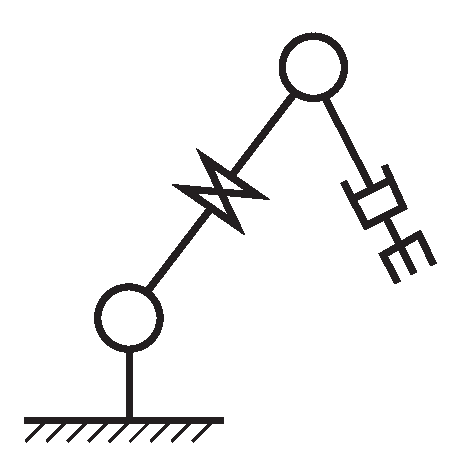
\includegraphics[width=0.5\textwidth]{RobotRep1.pdf}
          \caption{Conventional way of representing a manipulator. The circles show a rotation between the interconnected links on the plane of the paper. The cross symbol shows rotation on the link line. The square symbol is for prismatic joint. It represents change in length along the link line.}\label{FigConventionalRep}
        \end{figure}
        This kind of representation is clean and simple but doesn't give a complete view of the robot. Specially, with virtually zero link lengths, the visual representation can confuse someone new to the realm of robotic.

        Based on repeated experiments and to answer the weakness of contentional representation, let us define a new representation that encapsulates the basic idea of representation with some features of $D-H$ table. See Fig. \ref{FigMyRep}
        \begin{figure}
          \centering
          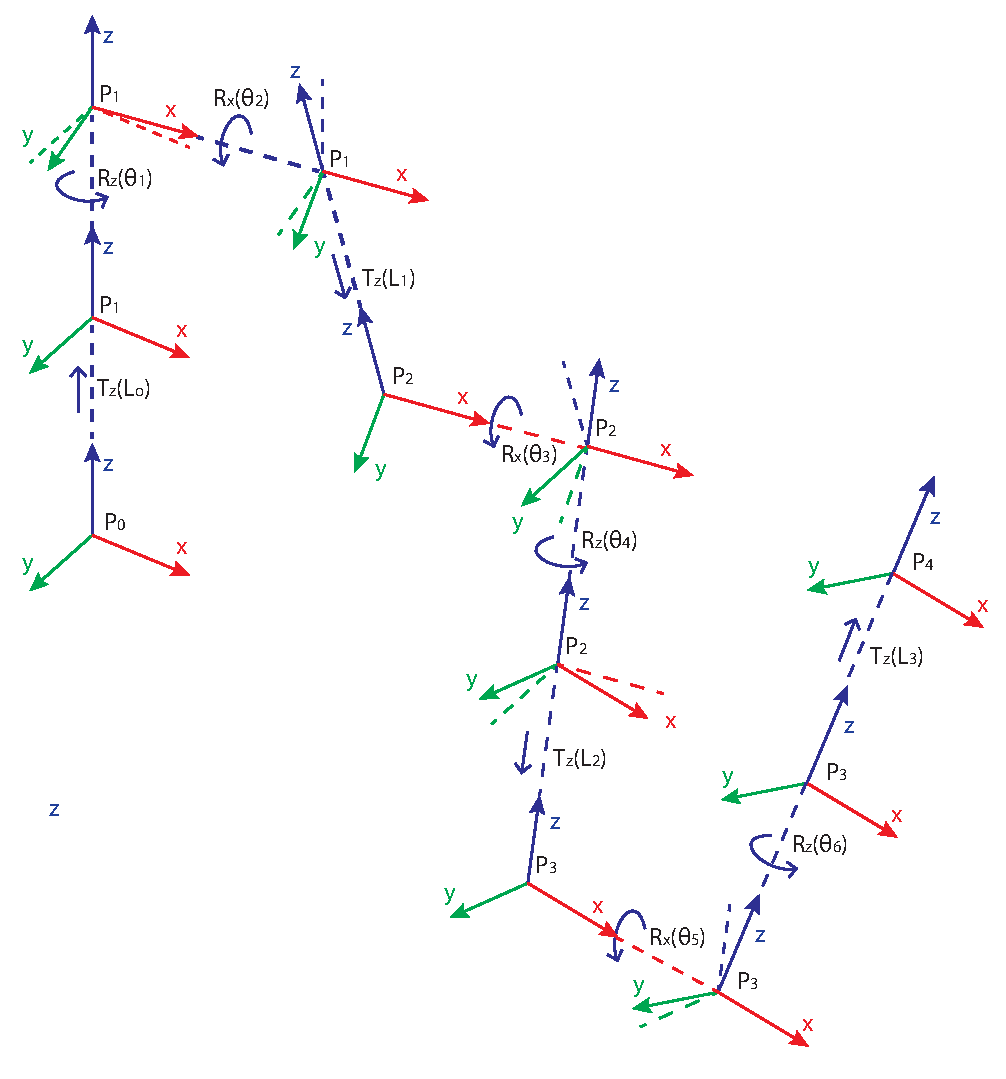
\includegraphics[width=0.8\textwidth]{MyRep.pdf}
          \caption{An example of \texttt{transformation frames} representation. This representation shows how a reference frame is linked to the previous using two basic transformation functions, $T_n$ and $R_n$ where n is the axis along or about which the transformation is performed. The schematic is drawn in the direction of $F0$ to $F_N$ ($N$ being the last frame) but can also be interpreted in reverse direction. One can easily see which transformations are required to convert one frame of reference to the other. One only needs to take one thing in account. When going in forward direction, all the transformations are applied as they are but while going back, each successive transformation is taken as inverse. For example, frame $F5$ can be achieved from frame $F3$ by applying two successive transformations: translation along $x$ of magnitude $L1$ and rotation about $x$ of magnitude $\theta_3$. However, to go to frame $F3$ from frame $F5$, one needs to apply two successive transformations: rotation about $x$ of magnitude $-\theta_3$ and translation along \texttt{x} of magnitude $-L1$. It should be noted that if a transformation changes the origin of the frame, the next frame has a different point shown at the center. This point is defined in the base frame.
          } \label{FigMyRep}
        \end{figure}

        Interestingly, this representation can't only represent physical manipulators, it can also represent abstract transformations. See Fig. \ref{FigEulerRep} which represents a target $P_t$ being represented as $z-x-z$ euler angles.

        \begin{figure}
          \centering
          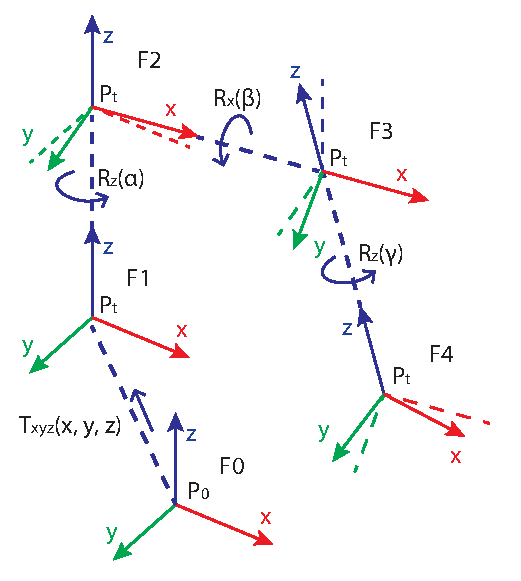
\includegraphics[width=0.6\textwidth]{EulerANgles.pdf}
          \caption{Three successive rotation $z-x-z$ and similar orders are call \texttt{Euler Angles Transformations}. A base Frame $F0$ is transformed though three translations and three euler rotations. This way, one can easily represent a target point to the robot which would have three extra components than $x$, $y$ and $z$; $\alpha$, $\beta$a and $\gamma$.
          } \label{FigEulerRep}
        \end{figure}

        Now, if one represents both target and the manipulator representation in a solved state, a closed loop representation can be formed which becomes extremely convenient in inverse kinematics. See Fig. \ref{FigCompleteRep} which exemplifies a closed loop \texttt{transformation frames} representation. It should be quite clear that once a closed loop is constructed, one can make transformations in any direction.

        \begin{figure}
          \centering
          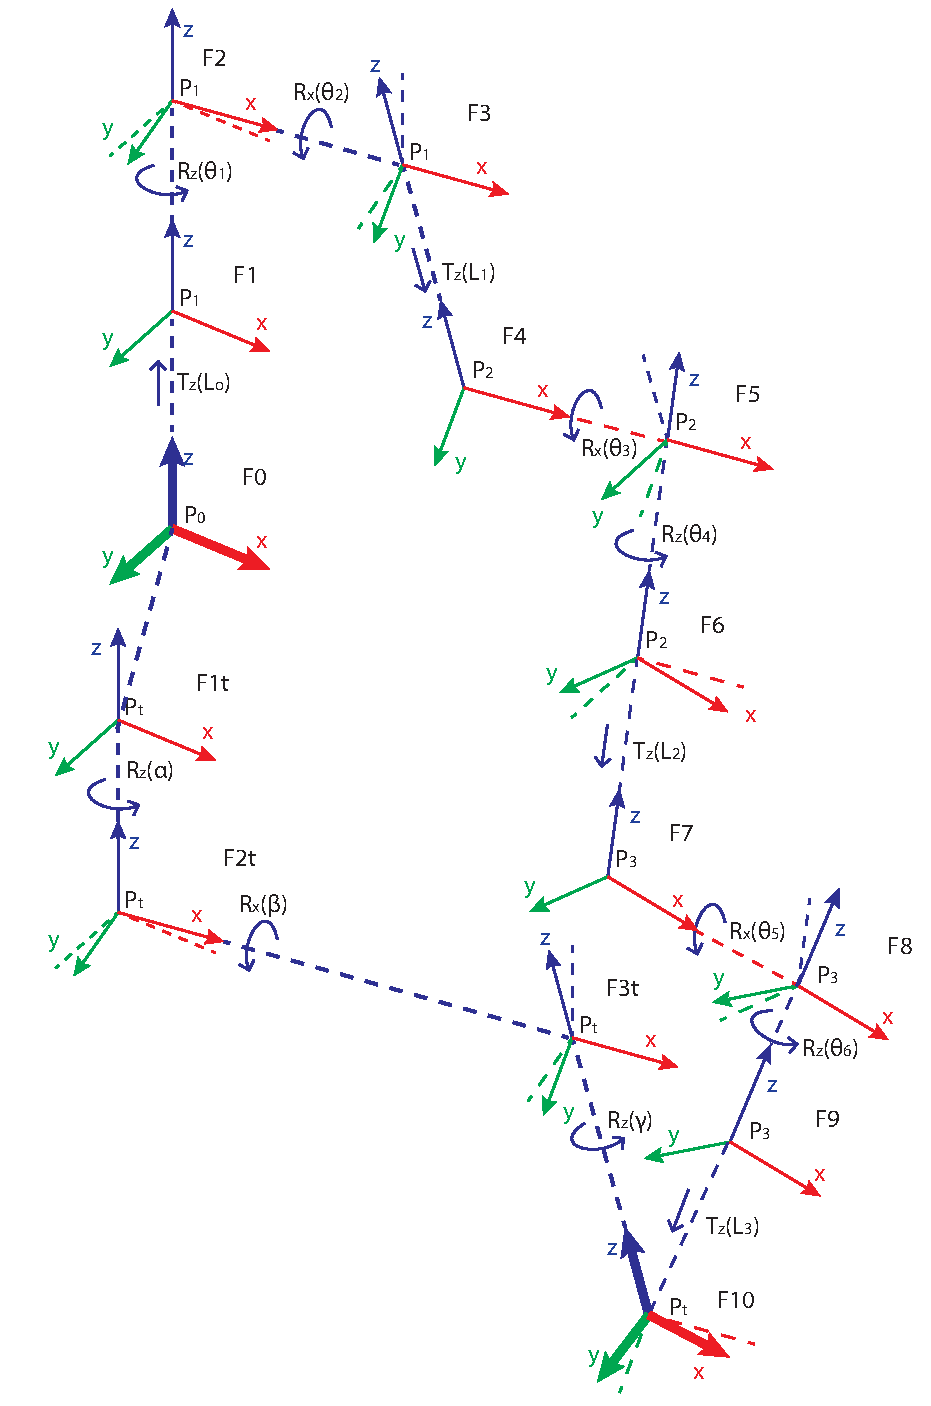
\includegraphics[width=0.9\textwidth]{CompleteRep.pdf}
          \caption{A manipulator along with a target represented in \texttt{transformation frames} representation. $F0$ corresponds to the base frame, $F0, F1, F2 ...$ represent the forward direction of the manipulator and $Ft0, Ft1, Ft2 ...$ represent the forward direction of the target. Both chains of transformations lead to a common reference frame eventually, the target frame of reference, or the end-effector frame of reference, $Ft$.
          } \label{FigCompleteRep}
        \end{figure}

        It is interesting to see that while doing a complete cycle transformation, one virtually transforms a frame through nothing! Also, if a $N-1$ frame transformation is applied in a $N$ frame closed loop, one can identify one last transformation quite easily by comparing the initial and the final frames. This method is called \texttt{Known Error Propagation} and will be used extensively in the inverse kinematics.

        Last, but not the least, of the usages of a closed loop representation is that some transformations can be skipped/swapped safely in order to simplify the loop. This can lead to finding further more unknown parameters using \texttt{Known Error Propagation}.

    }
    \subsection{Selecting a Configuration}
    {
        The configuration selected for this project is widely used by other engineers but the main inspiration behind choosing this configuration was a B.Sc. final year project of the \emph{Mechanical Engineering Department of U.E.T} of the batch $12$' with title, 'Design and Implementation of a $6$DoF Spot Welding Robot'. The project report presents a solution and describes all the forward and inverse kinematics. And all this, without using a regular transformation matrix! The effort in the current project takes some inspiration from the previous one and also elaborates not only the faults and issues with the previous but also the effectiveness of using transformation matrices.

        See Fig. \ref{FigCompleteRep} which represents this manipulator.

        In addition to these six degrees of freedom, we have attached a linear force control actuator along the end effector, since this actuator is responsible to keep the normal force under control, effectively, the robot solution remains the same as for six degrees. This scheme will be described later.
    }
    \subsection{Mathematical Modelling}
    {
        Using the new representation, properties of homogenous transformation matrices and basic highschool trigonometry,  I was able to calculate the unique and redundant solutions for the spherical manipulator. The process will be described later, but, summarily, the robot has two primary solutions: different joint positions yield the same end effector position and orientation. Connected to both solutions, are $4$ more secondary solutions which effect only the motor angles not the link locations.

        Finding out the mathematical equations is one job, verification is another. While dealing with three dimensional realm on a two dimensional paper, one can the solution but making small human errors on the way. It is quite easy to confuse the directions of rotations in a reference frames, resulting in typical errors which can be mitigated by some hit-and-trial of a few operations; adding or subtracting integral multiples of $\frac{\pi}{2}$ from the angles, inverting the length signs, inverting the angle directions. This can be done easily only if a representation tool is build alongside the robot modeling.
    }
    \subsection{Simulation and Analysis Solutions}
    {
        Even with a complete mathematical model, there are tasks which require the power of simulation either for design and planning or for the verification of the existing model. The tool used for this step is discussed in detail in the coming sections.
    }
}

    \subsection{Inverse and Forward Kinematics}
    Some of the motor angles are quite obvious. See the series of hand-sketched figures labelled with mask Fig. \texttt{RDn} in the subsequent pages which demonstrate how an inverse kinematic solution was discovered for this robot.

\subsection{The Calligraphy Job}
{
        Calligraphy is kind of art that finds its links in the, so called, technical areas. The write and discover new fonts on the way but one thing remains the same. Whatever the idea an artist has in his mind, has finally to be represented as Ink marks which, usually, are made flat head pens and rectangular paint brushes. The tool doesn't know what actually drives it, it only knows how it should react to the specific surface and specific kind of input.

        This is where we innovate: replace the hand of the artist with the robot. The mind that imagins/creates/discovers the art, however, cannot be replaced by the robot. Or even if it can be, it would be out of scope of this project. So, now we need to create two more interfaces: between the human and the robot and second, between the robot and the writing tool.

        For the first interface, we discovered a modified form of bezier curve, "the rotation supported bezier". Bezier curves were first reported in use by a French physicist, \texttt{Paul de Casteljau} using \texttt{de Casteljau's algorithm}. He used bezier splines to model the bodies of \texttt{Renault} cars in 1959. We, after all those years, have discovered how asymmetric pen rotation can be incorporated in the bezier curves to define language scripts that require an asymmetric pen tip.

        See Fig. \ref{FigBezier} which shows a screenshot of a bezier rotation curve constructed in \texttt{Drogon v2}.

        \begin{figure}
          \centering
          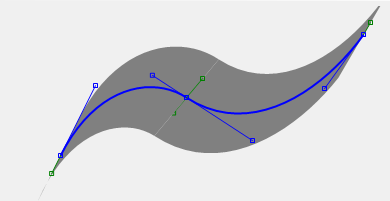
\includegraphics[width=0.7\textwidth]{bezier.png}
          \caption{A usual bezier spline has only two interlinked handles on a each anchor point which can control the shape of the curve before and after the anchor (shown blue). We have added a second (green) handle to each anchor which controls the rotation of the pen. Since the rotation handles act similar to the shapre handles, one can, in-effect, control change in rotation very accurately and smoothly.
          } \label{FigBezier}
        \end{figure}

    }
\subsection{Forward Kinematics} 